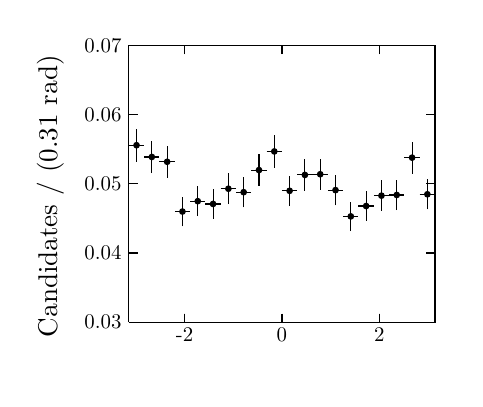
\begin{tikzpicture}
\pgfdeclareplotmark{cross} {
\pgfpathmoveto{\pgfpoint{-0.3\pgfplotmarksize}{\pgfplotmarksize}}
\pgfpathlineto{\pgfpoint{+0.3\pgfplotmarksize}{\pgfplotmarksize}}
\pgfpathlineto{\pgfpoint{+0.3\pgfplotmarksize}{0.3\pgfplotmarksize}}
\pgfpathlineto{\pgfpoint{+1\pgfplotmarksize}{0.3\pgfplotmarksize}}
\pgfpathlineto{\pgfpoint{+1\pgfplotmarksize}{-0.3\pgfplotmarksize}}
\pgfpathlineto{\pgfpoint{+0.3\pgfplotmarksize}{-0.3\pgfplotmarksize}}
\pgfpathlineto{\pgfpoint{+0.3\pgfplotmarksize}{-1.\pgfplotmarksize}}
\pgfpathlineto{\pgfpoint{-0.3\pgfplotmarksize}{-1.\pgfplotmarksize}}
\pgfpathlineto{\pgfpoint{-0.3\pgfplotmarksize}{-0.3\pgfplotmarksize}}
\pgfpathlineto{\pgfpoint{-1.\pgfplotmarksize}{-0.3\pgfplotmarksize}}
\pgfpathlineto{\pgfpoint{-1.\pgfplotmarksize}{0.3\pgfplotmarksize}}
\pgfpathlineto{\pgfpoint{-0.3\pgfplotmarksize}{0.3\pgfplotmarksize}}
\pgfpathclose
\pgfusepathqstroke
}
\pgfdeclareplotmark{cross*} {
\pgfpathmoveto{\pgfpoint{-0.3\pgfplotmarksize}{\pgfplotmarksize}}
\pgfpathlineto{\pgfpoint{+0.3\pgfplotmarksize}{\pgfplotmarksize}}
\pgfpathlineto{\pgfpoint{+0.3\pgfplotmarksize}{0.3\pgfplotmarksize}}
\pgfpathlineto{\pgfpoint{+1\pgfplotmarksize}{0.3\pgfplotmarksize}}
\pgfpathlineto{\pgfpoint{+1\pgfplotmarksize}{-0.3\pgfplotmarksize}}
\pgfpathlineto{\pgfpoint{+0.3\pgfplotmarksize}{-0.3\pgfplotmarksize}}
\pgfpathlineto{\pgfpoint{+0.3\pgfplotmarksize}{-1.\pgfplotmarksize}}
\pgfpathlineto{\pgfpoint{-0.3\pgfplotmarksize}{-1.\pgfplotmarksize}}
\pgfpathlineto{\pgfpoint{-0.3\pgfplotmarksize}{-0.3\pgfplotmarksize}}
\pgfpathlineto{\pgfpoint{-1.\pgfplotmarksize}{-0.3\pgfplotmarksize}}
\pgfpathlineto{\pgfpoint{-1.\pgfplotmarksize}{0.3\pgfplotmarksize}}
\pgfpathlineto{\pgfpoint{-0.3\pgfplotmarksize}{0.3\pgfplotmarksize}}
\pgfpathclose
\pgfusepathqfillstroke
}
\pgfdeclareplotmark{newstar} {
\pgfpathmoveto{\pgfqpoint{0pt}{\pgfplotmarksize}}
\pgfpathlineto{\pgfqpointpolar{44}{0.5\pgfplotmarksize}}
\pgfpathlineto{\pgfqpointpolar{18}{\pgfplotmarksize}}
\pgfpathlineto{\pgfqpointpolar{-20}{0.5\pgfplotmarksize}}
\pgfpathlineto{\pgfqpointpolar{-54}{\pgfplotmarksize}}
\pgfpathlineto{\pgfqpointpolar{-90}{0.5\pgfplotmarksize}}
\pgfpathlineto{\pgfqpointpolar{234}{\pgfplotmarksize}}
\pgfpathlineto{\pgfqpointpolar{198}{0.5\pgfplotmarksize}}
\pgfpathlineto{\pgfqpointpolar{162}{\pgfplotmarksize}}
\pgfpathlineto{\pgfqpointpolar{134}{0.5\pgfplotmarksize}}
\pgfpathclose
\pgfusepathqstroke
}
\pgfdeclareplotmark{newstar*} {
\pgfpathmoveto{\pgfqpoint{0pt}{\pgfplotmarksize}}
\pgfpathlineto{\pgfqpointpolar{44}{0.5\pgfplotmarksize}}
\pgfpathlineto{\pgfqpointpolar{18}{\pgfplotmarksize}}
\pgfpathlineto{\pgfqpointpolar{-20}{0.5\pgfplotmarksize}}
\pgfpathlineto{\pgfqpointpolar{-54}{\pgfplotmarksize}}
\pgfpathlineto{\pgfqpointpolar{-90}{0.5\pgfplotmarksize}}
\pgfpathlineto{\pgfqpointpolar{234}{\pgfplotmarksize}}
\pgfpathlineto{\pgfqpointpolar{198}{0.5\pgfplotmarksize}}
\pgfpathlineto{\pgfqpointpolar{162}{\pgfplotmarksize}}
\pgfpathlineto{\pgfqpointpolar{134}{0.5\pgfplotmarksize}}
\pgfpathclose
\pgfusepathqfillstroke
}
\definecolor{c}{rgb}{1,1,1};
\draw [color=c, fill=c] (5.1,4.72095) rectangle (9.9,9.16419);
\draw [color=c, fill=c] (5.772,5.43186) rectangle (9.66,8.94203);
\definecolor{c}{rgb}{0,0,0};
\draw [c] (5.772,5.43186) -- (5.772,8.94203) -- (9.66,8.94203) -- (9.66,5.43186) -- (5.772,5.43186);
\draw [c,line width=0.4] (5.8692,7.47145) -- (5.8692,7.67837);
\draw [c,line width=0.4] (5.8692,7.67837) -- (5.8692,7.88529);
\draw [c,line width=0.4] (5.772,7.67837) -- (5.8692,7.67837);
\draw [c,line width=0.4] (5.8692,7.67837) -- (5.9664,7.67837);
\foreach \P in {(5.8692,7.67837)}{\draw[mark options={color=c,fill=c},mark size=1.201201pt,mark=*,mark size=1pt] plot coordinates {\P};}
\draw [c,line width=0.4] (6.0636,7.32545) -- (6.0636,7.52919);
\draw [c,line width=0.4] (6.0636,7.52919) -- (6.0636,7.73292);
\draw [c,line width=0.4] (5.9664,7.52919) -- (6.0636,7.52919);
\draw [c,line width=0.4] (6.0636,7.52919) -- (6.1608,7.52919);
\foreach \P in {(6.0636,7.52919)}{\draw[mark options={color=c,fill=c},mark size=1.201201pt,mark=*,mark size=1pt] plot coordinates {\P};}
\draw [c,line width=0.4] (6.258,7.26535) -- (6.258,7.46776);
\draw [c,line width=0.4] (6.258,7.46776) -- (6.258,7.67016);
\draw [c,line width=0.4] (6.1608,7.46776) -- (6.258,7.46776);
\draw [c,line width=0.4] (6.258,7.46776) -- (6.3552,7.46776);
\foreach \P in {(6.258,7.46776)}{\draw[mark options={color=c,fill=c},mark size=1.201201pt,mark=*,mark size=1pt] plot coordinates {\P};}
\draw [c,line width=0.4] (6.4524,6.64772) -- (6.4524,6.83593);
\draw [c,line width=0.4] (6.4524,6.83593) -- (6.4524,7.02414);
\draw [c,line width=0.4] (6.3552,6.83593) -- (6.4524,6.83593);
\draw [c,line width=0.4] (6.4524,6.83593) -- (6.5496,6.83593);
\foreach \P in {(6.4524,6.83593)}{\draw[mark options={color=c,fill=c},mark size=1.201201pt,mark=*,mark size=1pt] plot coordinates {\P};}
\draw [c,line width=0.4] (6.6468,6.77631) -- (6.6468,6.96756);
\draw [c,line width=0.4] (6.6468,6.96756) -- (6.6468,7.15882);
\draw [c,line width=0.4] (6.5496,6.96756) -- (6.6468,6.96756);
\draw [c,line width=0.4] (6.6468,6.96756) -- (6.744,6.96756);
\foreach \P in {(6.6468,6.96756)}{\draw[mark options={color=c,fill=c},mark size=1.201201pt,mark=*,mark size=1pt] plot coordinates {\P};}
\draw [c,line width=0.4] (6.8412,6.74201) -- (6.8412,6.93246);
\draw [c,line width=0.4] (6.8412,6.93246) -- (6.8412,7.12291);
\draw [c,line width=0.4] (6.744,6.93246) -- (6.8412,6.93246);
\draw [c,line width=0.4] (6.8412,6.93246) -- (6.9384,6.93246);
\foreach \P in {(6.8412,6.93246)}{\draw[mark options={color=c,fill=c},mark size=1.201201pt,mark=*,mark size=1pt] plot coordinates {\P};}
\draw [c,line width=0.4] (7.0356,6.93067) -- (7.0356,7.12552);
\draw [c,line width=0.4] (7.0356,7.12552) -- (7.0356,7.32036);
\draw [c,line width=0.4] (6.9384,7.12552) -- (7.0356,7.12552);
\draw [c,line width=0.4] (7.0356,7.12552) -- (7.1328,7.12552);
\foreach \P in {(7.0356,7.12552)}{\draw[mark options={color=c,fill=c},mark size=1.201201pt,mark=*,mark size=1pt] plot coordinates {\P};}
\draw [c,line width=0.4] (7.23,6.88779) -- (7.23,7.08164);
\draw [c,line width=0.4] (7.23,7.08164) -- (7.23,7.2755);
\draw [c,line width=0.4] (7.1328,7.08164) -- (7.23,7.08164);
\draw [c,line width=0.4] (7.23,7.08164) -- (7.3272,7.08164);
\foreach \P in {(7.23,7.08164)}{\draw[mark options={color=c,fill=c},mark size=1.201201pt,mark=*,mark size=1pt] plot coordinates {\P};}
\draw [c,line width=0.4] (7.4244,7.16234) -- (7.4244,7.36245);
\draw [c,line width=0.4] (7.4244,7.36245) -- (7.4244,7.56256);
\draw [c,line width=0.4] (7.3272,7.36245) -- (7.4244,7.36245);
\draw [c,line width=0.4] (7.4244,7.36245) -- (7.5216,7.36245);
\foreach \P in {(7.4244,7.36245)}{\draw[mark options={color=c,fill=c},mark size=1.201201pt,mark=*,mark size=1pt] plot coordinates {\P};}
\draw [c,line width=0.4] (7.6188,7.39415) -- (7.6188,7.59939);
\draw [c,line width=0.4] (7.6188,7.59939) -- (7.6188,7.80463);
\draw [c,line width=0.4] (7.5216,7.59939) -- (7.6188,7.59939);
\draw [c,line width=0.4] (7.6188,7.59939) -- (7.716,7.59939);
\foreach \P in {(7.6188,7.59939)}{\draw[mark options={color=c,fill=c},mark size=1.201201pt,mark=*,mark size=1pt] plot coordinates {\P};}
\draw [c,line width=0.4] (7.8132,6.90494) -- (7.8132,7.09919);
\draw [c,line width=0.4] (7.8132,7.09919) -- (7.8132,7.29344);
\draw [c,line width=0.4] (7.716,7.09919) -- (7.8132,7.09919);
\draw [c,line width=0.4] (7.8132,7.09919) -- (7.9104,7.09919);
\foreach \P in {(7.8132,7.09919)}{\draw[mark options={color=c,fill=c},mark size=1.201201pt,mark=*,mark size=1pt] plot coordinates {\P};}
\draw [c,line width=0.4] (8.0076,7.10227) -- (8.0076,7.30103);
\draw [c,line width=0.4] (8.0076,7.30103) -- (8.0076,7.49978);
\draw [c,line width=0.4] (7.9104,7.30103) -- (8.0076,7.30103);
\draw [c,line width=0.4] (8.0076,7.30103) -- (8.1048,7.30103);
\foreach \P in {(8.0076,7.30103)}{\draw[mark options={color=c,fill=c},mark size=1.201201pt,mark=*,mark size=1pt] plot coordinates {\P};}
\draw [c,line width=0.4] (8.202,7.11085) -- (8.202,7.3098);
\draw [c,line width=0.4] (8.202,7.3098) -- (8.202,7.50875);
\draw [c,line width=0.4] (8.1048,7.3098) -- (8.202,7.3098);
\draw [c,line width=0.4] (8.202,7.3098) -- (8.2992,7.3098);
\foreach \P in {(8.202,7.3098)}{\draw[mark options={color=c,fill=c},mark size=1.201201pt,mark=*,mark size=1pt] plot coordinates {\P};}
\draw [c,line width=0.4] (8.3964,6.91352) -- (8.3964,7.10797);
\draw [c,line width=0.4] (8.3964,7.10797) -- (8.3964,7.30242);
\draw [c,line width=0.4] (8.2992,7.10797) -- (8.3964,7.10797);
\draw [c,line width=0.4] (8.3964,7.10797) -- (8.4936,7.10797);
\foreach \P in {(8.3964,7.10797)}{\draw[mark options={color=c,fill=c},mark size=1.201201pt,mark=*,mark size=1pt] plot coordinates {\P};}
\draw [c,line width=0.4] (8.5908,6.58773) -- (8.5908,6.7745);
\draw [c,line width=0.4] (8.5908,6.7745) -- (8.5908,6.96128);
\draw [c,line width=0.4] (8.4936,6.7745) -- (8.5908,6.7745);
\draw [c,line width=0.4] (8.5908,6.7745) -- (8.688,6.7745);
\foreach \P in {(8.5908,6.7745)}{\draw[mark options={color=c,fill=c},mark size=1.201201pt,mark=*,mark size=1pt] plot coordinates {\P};}
\draw [c,line width=0.4] (8.7852,6.71629) -- (8.7852,6.90613);
\draw [c,line width=0.4] (8.7852,6.90613) -- (8.7852,7.09597);
\draw [c,line width=0.4] (8.688,6.90613) -- (8.7852,6.90613);
\draw [c,line width=0.4] (8.7852,6.90613) -- (8.8824,6.90613);
\foreach \P in {(8.7852,6.90613)}{\draw[mark options={color=c,fill=c},mark size=1.201201pt,mark=*,mark size=1pt] plot coordinates {\P};}
\draw [c,line width=0.4] (8.9796,6.8449) -- (8.9796,7.03776);
\draw [c,line width=0.4] (8.9796,7.03776) -- (8.9796,7.23062);
\draw [c,line width=0.4] (8.8824,7.03776) -- (8.9796,7.03776);
\draw [c,line width=0.4] (8.9796,7.03776) -- (9.0768,7.03776);
\foreach \P in {(8.9796,7.03776)}{\draw[mark options={color=c,fill=c},mark size=1.201201pt,mark=*,mark size=1pt] plot coordinates {\P};}
\draw [c,line width=0.4] (9.174,6.85348) -- (9.174,7.04654);
\draw [c,line width=0.4] (9.174,7.04654) -- (9.174,7.2396);
\draw [c,line width=0.4] (9.0768,7.04654) -- (9.174,7.04654);
\draw [c,line width=0.4] (9.174,7.04654) -- (9.2712,7.04654);
\foreach \P in {(9.174,7.04654)}{\draw[mark options={color=c,fill=c},mark size=1.201201pt,mark=*,mark size=1pt] plot coordinates {\P};}
\draw [c,line width=0.4] (9.3684,7.31687) -- (9.3684,7.52041);
\draw [c,line width=0.4] (9.3684,7.52041) -- (9.3684,7.72396);
\draw [c,line width=0.4] (9.2712,7.52041) -- (9.3684,7.52041);
\draw [c,line width=0.4] (9.3684,7.52041) -- (9.4656,7.52041);
\foreach \P in {(9.3684,7.52041)}{\draw[mark options={color=c,fill=c},mark size=1.201201pt,mark=*,mark size=1pt] plot coordinates {\P};}
\draw [c,line width=0.4] (9.5628,6.86206) -- (9.5628,7.05532);
\draw [c,line width=0.4] (9.5628,7.05532) -- (9.5628,7.24857);
\draw [c,line width=0.4] (9.4656,7.05532) -- (9.5628,7.05532);
\draw [c,line width=0.4] (9.5628,7.05532) -- (9.66,7.05532);
\foreach \P in {(9.5628,7.05532)}{\draw[mark options={color=c,fill=c},mark size=1.201201pt,mark=*,mark size=1pt] plot coordinates {\P};}
\draw [c,line width=0.4] (5.772,5.43186) -- (9.66,5.43186);
\draw [anchor= east] (9.66,4.93422) node[scale=0.979298, rotate=0]{$\phihel$};
\draw [c,line width=0.4] (6.47841,5.53984) -- (6.47841,5.43186);
\draw [c,line width=0.4] (7.716,5.53984) -- (7.716,5.43186);
\draw [c,line width=0.4] (8.95359,5.53984) -- (8.95359,5.43186);
\draw [c,line width=0.4] (6.47841,5.53984) -- (6.47841,5.43186);
\draw [c,line width=0.4] (8.95359,5.53984) -- (8.95359,5.43186);
\draw [anchor=base] (6.47841,5.19193) node[scale=0.753306, rotate=0]{-2};
\draw [anchor=base] (7.716,5.19193) node[scale=0.753306, rotate=0]{0};
\draw [anchor=base] (8.95359,5.19193) node[scale=0.753306, rotate=0]{2};
\draw [c,line width=0.4] (5.772,8.94203) -- (9.66,8.94203);
\draw [c,line width=0.4] (6.47841,8.83406) -- (6.47841,8.94203);
\draw [c,line width=0.4] (7.716,8.83406) -- (7.716,8.94203);
\draw [c,line width=0.4] (8.95359,8.83406) -- (8.95359,8.94203);
\draw [c,line width=0.4] (6.47841,8.83406) -- (6.47841,8.94203);
\draw [c,line width=0.4] (8.95359,8.83406) -- (8.95359,8.94203);
\draw [c,line width=0.4] (5.772,5.43186) -- (5.772,8.94203);
\draw [anchor= east] (4.7736,8.94203) node[scale=0.979298, rotate=90]{Candidates / (0.31 rad)};
\draw [c,line width=0.4] (5.88576,5.43186) -- (5.772,5.43186);
\draw [c,line width=0.4] (5.88576,6.30941) -- (5.772,6.30941);
\draw [c,line width=0.4] (5.88576,7.18695) -- (5.772,7.18695);
\draw [c,line width=0.4] (5.88576,8.06449) -- (5.772,8.06449);
\draw [c,line width=0.4] (5.88576,8.94203) -- (5.772,8.94203);
\draw [anchor= east] (5.772,5.43186) node[scale=0.753306, rotate=0]{0.03};
\draw [anchor= east] (5.772,6.30941) node[scale=0.753306, rotate=0]{0.04};
\draw [anchor= east] (5.772,7.18695) node[scale=0.753306, rotate=0]{0.05};
\draw [anchor= east] (5.772,8.06449) node[scale=0.753306, rotate=0]{0.06};
\draw [anchor= east] (5.772,8.94203) node[scale=0.753306, rotate=0]{0.07};
\draw [c,line width=0.4] (9.66,5.43186) -- (9.66,8.94203);
\draw [c,line width=0.4] (9.54624,5.43186) -- (9.66,5.43186);
\draw [c,line width=0.4] (9.54624,6.30941) -- (9.66,6.30941);
\draw [c,line width=0.4] (9.54624,7.18695) -- (9.66,7.18695);
\draw [c,line width=0.4] (9.54624,8.06449) -- (9.66,8.06449);
\draw [c,line width=0.4] (9.54624,8.94203) -- (9.66,8.94203);
\end{tikzpicture}
